\documentclass[a4paper, 12pt, titlepage, fleqn]{article}

%Taal: Nederlands ("Inhoudsopgave", "Hoofdstuk",...)
\usepackage{graphicx}
\usepackage{subcaption}
\usepackage{amsmath, amssymb, textcomp, mathtools}
\usepackage{geometry}
	\geometry{a4paper, left=20mm, right=20mm, top=20mm, bottom=20mm}
\setlength{\mathindent}{1cm}
%Hyperlinks
\usepackage{hyperref}
\usepackage{subcaption}

%Opmaak hyperlinks
\hypersetup{colorlinks=false,	urlcolor=cyan,pdfborder=0 0 0}
\usepackage[framed,numbered,autolinebreaks,useliterate]{mcode}
%geen indents
\setlength\parindent{0pt}
\usepackage{listings}
\lstset{
language=Matlab, % choose the language of the code
%basicstyle=10pt, % the size of the fonts that are used for the code
numbers=left, % where to put the line-numbers
numberstyle=\footnotesize, % the size of the fonts that are used for the line-numbers
stepnumber=1, % the step between two line-numbers. If it's 1 each line will be numbered
numbersep=5pt, % how far the line-numbers are from the code
%backgroundcolor=\color{grey}, % choose the background color. You must add \usepackage{color}
showspaces=false, % show spaces adding particular underscores
showstringspaces=false, % underline spaces within strings
showtabs=false, % show tabs within strings adding particular underscores
frame=single, % adds a frame around the code
%tabsize=2, % sets default tabsize to 2 spaces
captionpos=b, % sets the caption-position to bottom
breaklines=true, % sets automatic line breaking
breakatwhitespace=false, % sets if automatic breaks should only happen at whitespace
escapeinside={\%*}{*)} % if you want to add a comment within your code
}

\captionsetup{
   font=small,          % Select font size
   margin=3em,          % Margin, left and right
   tableposition=top    % Formatting for captions above tables
}

\newcounter{nalg} % defines algorithm counter for chapter-level
%\renewcommand{\thenalg}{\thechapter .\arabic{nalg}} %defines appearance of the algorithm counter
\DeclareCaptionLabelFormat{algocaption}{Algoritme \thenalg} % defines a new caption label as Algorithm x.y

\lstnewenvironment{algorithm}[1][] %defines the algorithm listing environment
{   
    \refstepcounter{nalg} %increments algorithm number
    \captionsetup{labelformat=algocaption} %defines the caption setup for: it ises label format as the declared caption label above and makes label and caption text to be separated by a ':'
    \lstset{ %this is the stype
        mathescape=true,
        frame=tblr,
        numbers=left, 
        numberstyle=\tiny,
        basicstyle=\scriptsize, 
        keywordstyle=\color{black}\bfseries,
        keywords={,input, output, return, datatype, function, in, if, else, foreach, while, begin, end, for, do, } %add the keywords you want, or load a language as Rubens explains in his comment above.
        numbers=left,
        xleftmargin=.04\textwidth,
        #1 % this is to add specific settings to an usage of this environment (for instnce, the caption and referable label)
    }
}
{}

\usepackage[dutch]{babel}
\begin{document}

\title{\textbf{Numerieke Modellering en Benadering: Eigenwaardeproblemen en iteratieve methoden}}
\author{Sander Prenen, r0701014}

\date{20 mei 2020}
\begin{titlepage}
	\maketitle
	\thispagestyle{empty}
\end{titlepage}

\newpage
\tableofcontents
\listoffigures
\newpage

\section{Inleiding}
In dit verslag worden verschillenden methodes bestudeerd om eigenwaardenproblemen op te lossen. In sectie \ref{sec:gelijktijdige iteratie} wordt de gelijktijdige iteratie bekeken en wordt het algoritme aangepast om de eigenwaarden te vinden dicht bij een gegeven waarde. In sectie \ref{sec:inverse iteratie} wordt zowel de inverse iteratie als de Rayleigh-iteratie bekeken en worden ze vergeleken. Vervolgens wordt in sectie \ref{sec: jacobi} de Jacobi-methode bekeken en deze methode wordt in MATLAB ge\"implementeerd. Ten slotte wordt in sectie \ref{sec: geconjugeerde gradienten} de methode van de geconjugeerde gradi\"enten bekeken en de bijbehorende convergentiesnelheid.

\section{Gelijktijdige iteratie}\label{sec:gelijktijdige iteratie}
\underline{\textbf{Opgave 1a}}\\

Bij gelijktijdige iteratie of 'simultaneous iteration' wordt de methode van de machten toegepast op $p$ kolommen tegelijk. De methode convergeert naar de $p$ grootste eigenwaarden en de bijhorende eigenvectoren. Door de methode licht te wijzigen, kunnen de $p$ eigenwaarden van een symmetrische niet-singuliere matrix $A$, die het dichtst bij een gegeven waarde $\mu$ liggen, bepaald worden. Hiervoor wordt verondersteld dat $\mu$ geen eigenwaarde is van $A$. Het algoritme kan hiervoor gebruikt worden als de $p$ eigenwaarden het dichtst bij $\mu$ ook de $p$ grootste eigenwaarden zijn. Hiervoor kan gezorgd worden door de matrix $A$ te vervangen door $A - \mu I$. Deze matrix heeft eigenwaarden die $\mu$ lager liggen dan de eigenwaarden van de originele matrix $A$. Dit kan als volgt worden ingezien. De originele eigenwaarden $\lambda_o$ zijn de oplossing van volgende vergelijking:
\begin{align*}
\det (A-\lambda_o I) = 0
\end{align*}
De eigenwaarden $\lambda_n$ van de nieuwe matrix zijn de oplossingen van onderstaande vergelijking:
\begin{align*}
\det (A - \mu I - \lambda_n I) = 0 \Leftrightarrow \det(A -(\mu + \lambda_n)I) = 0
\end{align*}
Dit leidt tot volgende gelijkheid $\lambda_o = \mu + \lambda_n$. Dit betekent dat de nieuwe eigenwaarden $\lambda_n$ inderdaad $\mu$ lager liggen dan de originele eigenwaarden $\lambda_o$.\\
Nu zijn de $p$ gezochte eigenwaarden de kleinste van alle eigenwaarden. Om er voor te zorgen dat ze de $p$ grootste eigenwaarden worden, wordt de inverse matrix gebruikt. De inverse matrix heeft namelijk als eigenwaarden de reciproke eigenwaarden van de originele matrix.
\begin{align*}
Ax &= \lambda x\\
A\frac{1}{\lambda}x &= x\\
A^{-1}A\frac{1}{\lambda}x &= A^{-1}x\\
\frac{1}{\lambda}x &= A^{-1}x
\end{align*}
Nu zijn de $p$ eigenwaarden die het dichtst bij $\mu$ liggen de grootste eigenwaarden van de matrix en kan de methode van gelijktijdige iteratie gebruikt worden. In algoritme \ref{alg:gelijktijdige iteratie} kan de pseudocode voor deze methode gevonden worden. De kolommen van $\hat{Q}^{(k)}$ convergeren naar de eigenvectoren horende bij de eigenwaarden. Op deze kolommen $q^{(k)}$ wordt het Rayleigh quoti\"ent toegepast om de bijbehorende eigenwaarden te benaderen.

\begin{algorithm}[caption={Gelijktijdige iteratie}, label={alg:gelijktijdige iteratie}]
Kies $\hat{Q}^{(0)} \in \mathbb{R}^{m\times n}$ met orthonormale kolommen
for $k = 1,2,\ldots$ do
	$Z = (A-\mu I)^{-1}\hat{Q}^{(k-1)}$
	$\hat{Q}^{(k)}\hat{R}^{(k)} = Z$
	$\lambda^{(k)} = q^{(k)^\intercal}(A -\mu I)^{-1}q^{(k)}$
end
\end{algorithm}

\underline{\textbf{Opgave 1b}}\\

Wanneer twee eigenwaarden even ver van $\mu$ verwijderd liggen, kan de methode in sommige gevallen niet convergeren. De waarde in de verschillende iteratiestappen van de berkende eigenwaarde $\lambda^{(k)}$ voldoet namelijk aan de volgende gelijkheid:
\begin{align*}
|\lambda^{(k)} - \lambda_J| = \mathcal{O}\left(\left|\frac{\mu - \lambda_J}{\mu - \lambda_K}\right|^{2k}\right)
\end{align*} 
Als de eigenwaarden $\lambda_J$ en $\lambda_K$, die het dichtst bij $\mu$ liggen, gelijk zijn convergeert de methode niet. Door de eindige precisie van een computer zal de deling in het rechterlid van de vergelijking bijna nooit exact 1 geven. Hierdoor zal het in de meeste gevallen wel convergeren.

\section{Inverse iteratie en Rayleigh quoti\"ent iteratie}\label{sec:inverse iteratie}
\subsection{Rayleigh quoti\"ent iteratie}
\underline{\textbf{Opgave 2a}}\\

Om eigenwaarden te benaderen kan de Rayleigh quoti\"ent iteratie gebruikt worden. Deze methode convergeert kubisch naar de correct waarde. Elke iteratiestap moet het volgende stelsel opgelost worden:
\begin{align*}
(A - \lambda^{(k-1)}I)w = v^{(k-1)}
\end{align*}
Indien de benaderende eigenwaarde $\lambda^{(k-1)}$ dicht in de buurt komt van de exacte eigenwaarde, wordt dit stelsel meer en meer singulier. Hierdoor kan de oplossing $w$ van dit stelsel opblazen. Dit vormt echter geen proleem voor de iteratie aangezien $w$ genormeerd wordt. Enkel de richting van de vector $w$ is dus belangrijk en deze wordt niet veranderd.\\

\underline{\textbf{Opgave 2b}}\\

Er kan aangetoond worden dat voor een matrix $A \in \mathbb{R}^{n\times n}$ en een vector $x \in \mathbb{R}^{n \times 1}$, met $x$ een benadering voor een eigenvector van $A$, de oplossing $\rho \in \mathbb{R}$ van het volgende minimalisatieprobleem
\begin{align*}
\min_{\rho \in \mathbb{R}} \| Ax - \rho x\|_2
\end{align*}
overeenkomt met het Rayleigh quoti\"ent van $x$. \\

De functie $f(\rho) = \|Ax-\rho x\|_2 = (Ax-\rho x)^\intercal(Ax-\rho x)$ moet geminimaliseerd worden.\\ De afgeleide $f'(\rho)$ moet dus nul zijn.
\begin{align*}
(Ax-\rho x)^\intercal (Ax-\rho x) &= x^\intercal A^\intercal Ax - x^\intercal A^\intercal\rho x - x^\intercal\rho Ax + \rho^2x^\intercal x\\
&= x^\intercal A^\intercal Ax -2\rho x^\intercal Ax + \rho^2x^\intercal x
\end{align*}
Deze vergelijking afleiden naar $\rho$ en gelijk stellen aan nul geeft volgende uitdrukking:
\begin{align*}
-2x^\intercal Ax + 2\rho x^\intercal x = 0 \Leftrightarrow \rho = \frac{x^\intercal Ax}{x^\intercal x}
\end{align*}
Deze laatste uitdrukking is inderdaad het Rayleigh quoti\"ent.

\subsection{Vergelijking inverse iteratie en Rayleigh quoti\"ent iteratie}
\underline{\textbf{Opgave 3}}\\

Door de kubische convergentie van de Rayleigh quoti\"ent iteratie heeft deze methode vaak de voorkeur over de inverse iteratie. Toch zijn er ook gevallen waar de inverse iteratie de voorkeur geniet. Er worden in deze tekst twee gevallen besproken:
\begin{itemize}
\item \underline{De matrix $A \in \mathbb{R}^{m\times m}$ is (zeer) groot:} In elke iteratiestap van de Rayleigh quoti\"ent iteratie moet een nieuwe matrix ge\"inverteerd worden. Hierdoor zijn er $\mathcal{O}(m^3)$ flops nodig per stap. Voor de inverse iteratie moet er een lineair stelsel worden opgelost in elke stap. Dit lijkt op het eerste zicht $\mathcal{O}(m^3)$ flops te vragen, maar als de matrix $A$ op $QR$-gefactoriseerd is, vermindert het aantal flops naar $\mathcal{O}(m^2)$. Hierdoor is de inverse iteratie beter geschikt voor grote matrices.
\item \underline{De spectrale eigenschappen van $A$ zijn nauwelijks gekend}: Het doel is om een eigenpaar te vinden die het dichtst bij $\mu \in \mathbb{R}$ ligt, maar een goede startwaarde voor de eigenvector is niet gekend. De Rayleigh quoti\"ent iteratie vertrekt van een startwaarde van een eigenvector. Deze startwaarde is hier niet gekend dus is de inverse iteratie, die vertrekt van een startwaarde voor de eigenwaarde, beter geschikt.
\end{itemize}

\section{Jacobi-methode}\label{sec: jacobi}
De Jacobi-methode steunt op de diagonalisatie van $2 \times 2$ symmetrische matrices met behulp van een orthogonale matrix $J$,
\begin{align}\label{eq:jacobi}
J^T\left[\begin{matrix}
a &d\\
d &b
\end{matrix}\right]J = \left[ \begin{matrix}
\neq 0 &0\\
0 &\neq 0
\end{matrix}\right]
\end{align}
Hierbij wordt de orthogonale matrix $J$ gedefinieerd als een rotatie-matrix:
\begin{align}\label{eq:cs}
J  = \left[\begin{matrix}
c &s\\
-s &c
\end{matrix}\right]
\end{align}

\subsection{De co\"effici\"enten $c$ en $s$}
\underline{\textbf{Opgave 4}}\\

In deze sectie worden de co\"effici\"enten $c$ en $s$ van de matrix $J$ uit vergelijking (\ref{eq:cs}) bepaald zodat (\ref{eq:jacobi}) geldt. Aangezien $J$ een rotatie-matrix is, is de determinant van $j$ gelijk aan 1.
\begin{align*}
\det J = c^2 + s^2 = 1
\end{align*}
Volgende oplossing is een oplossing van het stelsel:
\begin{align*}
\begin{cases}
c = \cos(\theta)\\
s = \sin(\theta)
\end{cases}
\end{align*}
Indien de niet-diagonaal elementen in vergelijking~(\ref{eq:jacobi}) worden bepaald, wordt volgende uitdrukking verkregen:
\begin{align*}
\frac{1}{2}\sin(2\theta)(a-b) + d\cos(2\theta) = 0
\end{align*}
Hieruit kan $\theta$ gehaald worden:
\begin{align}\label{eq:theta}
\theta = \frac{1}{2}\arctan\left(\frac{2d}{b-a}\right)
\end{align}
Als $a$ gelijk is aan $b$ wordt $\theta$ gelijk aan $\frac{\pi}{4}$ aangezien voor deze hoek de boogtangens oneindig wordt.

\subsection{Eigenwaardeontbinding}
\underline{\textbf{Opgave 5}}\\

De Jacobi methode kan gebruikt worden om de eigenwaarden ontbinding $VDV^T$ van een symmetrische matrix $A$ te berekenen. Hierbij is $D$ een diagonaalmatrix die de eigenwaarden bevat en $V$ een orthoognale matrix met de overeenkomstige eigenvectoren. In algoritme~\ref{alg:jacobi-methode} kan de pseudo-code voor dit algoritme gevonden worden. In dit algoritme wordt de $sweep$-methode gebruikt die in het handboek beschreven staat.

\begin{algorithm}[caption={Jacobi-methode}, label={alg:jacobi-methode}]
$n = \text{size}(A)$
$V = I_n$
$\text{error} = \|R_A\|_F$
while error > tol do
	neem het volgende element van de $sweep$
	definieer $a$, $b$, $d$
	bepaal $\theta$ met vergelijking (3)
	stel de Jacobimatrix $J$ op
	$A = J^TAJ$
	$V = VJ$
	$\text{error} = \|R_A\|_F$
end
\end{algorithm}

Het algoritme wordt vervolgens ge\"implementeerd in MATLAB. In listing \ref{lst:jacobi} kan de code hiervan gevonden worden.\\

\underline{\textbf{Opgave 6}}\\

 Vervolgens wordt het algoritme getest op een $35\times35$ matrix. De frobeniusnorm $\|R_A\|_F$ van de bovendriehoekselementen wordt na elke iteratiestap berekend. In figuur~\ref{fig:jacobiFout} wordt $\|R_A\|_F$ afgebeeld in functie van het aantal iteratiestappen. De omcirkelde waarden zijn de iteratiestappen waarbij een volledige $sweep$ gedaan is. Het kruisje duid aan waar de norm onder de tolerantiegrens van $10^{-16}$ komt, hier is niet noodzakelijk een volledige $sweep$ gedaan. Er zijn in totaal dus acht volledige $sweeps$ nodig om de opgelegde tolerantie van $10^{-16}$ te bereiken. Dat wil zeggen dat de convergentie beter dan lineair is zoals in het handboek beschreven staat. In figuur~\ref{fig:sweeps} wordt de forbeniusnorm weergegeven in functie van het aantal $sweeps$. 

\begin{figure}
 \centering
 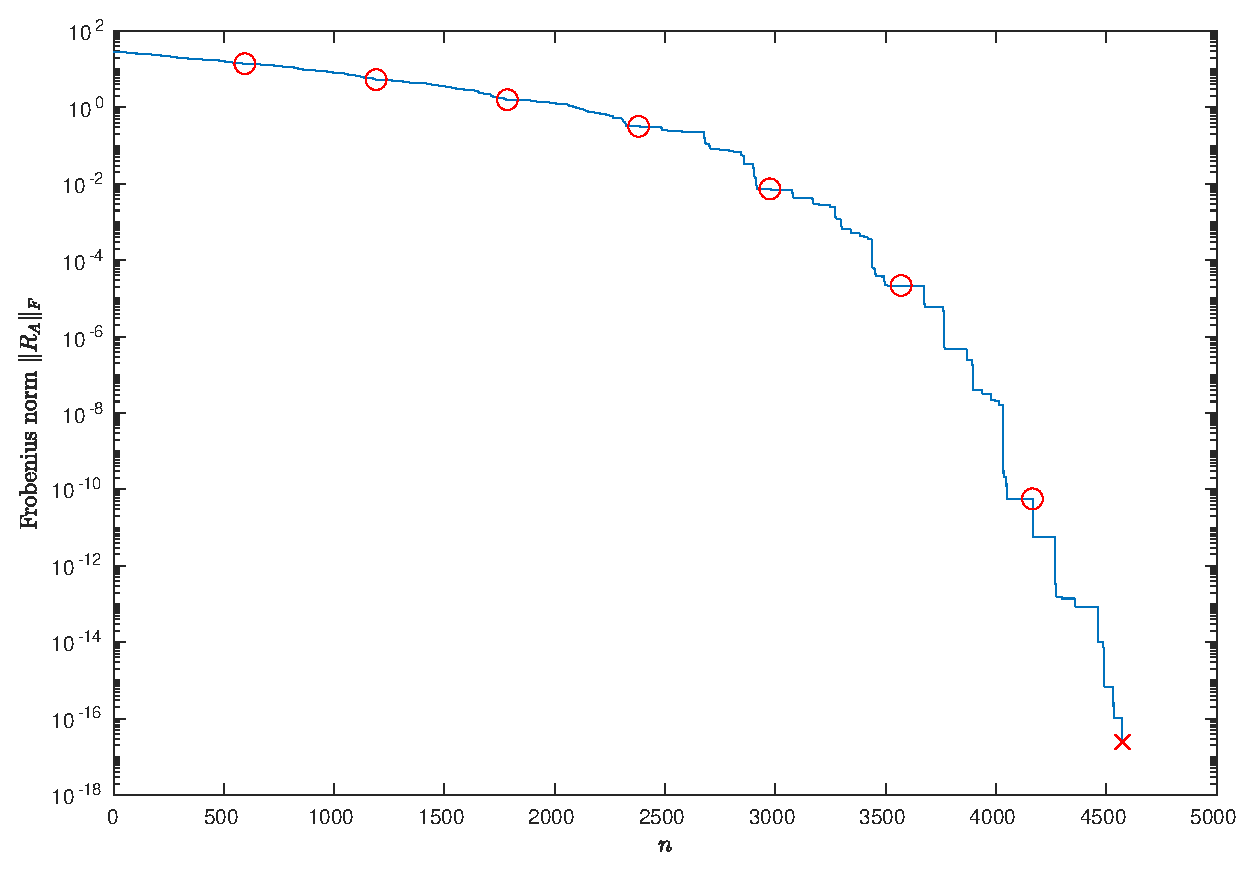
\includegraphics[scale=0.55]{../Afbeeldingen/fout-jacobi.eps}
 \caption{Frobeniusnorm $\|R_A\|_F$ in functie van het aantal iteratiestappen $n$}
 \label{fig:jacobiFout}
 \end{figure} 
 
 \begin{figure}
 \centering
 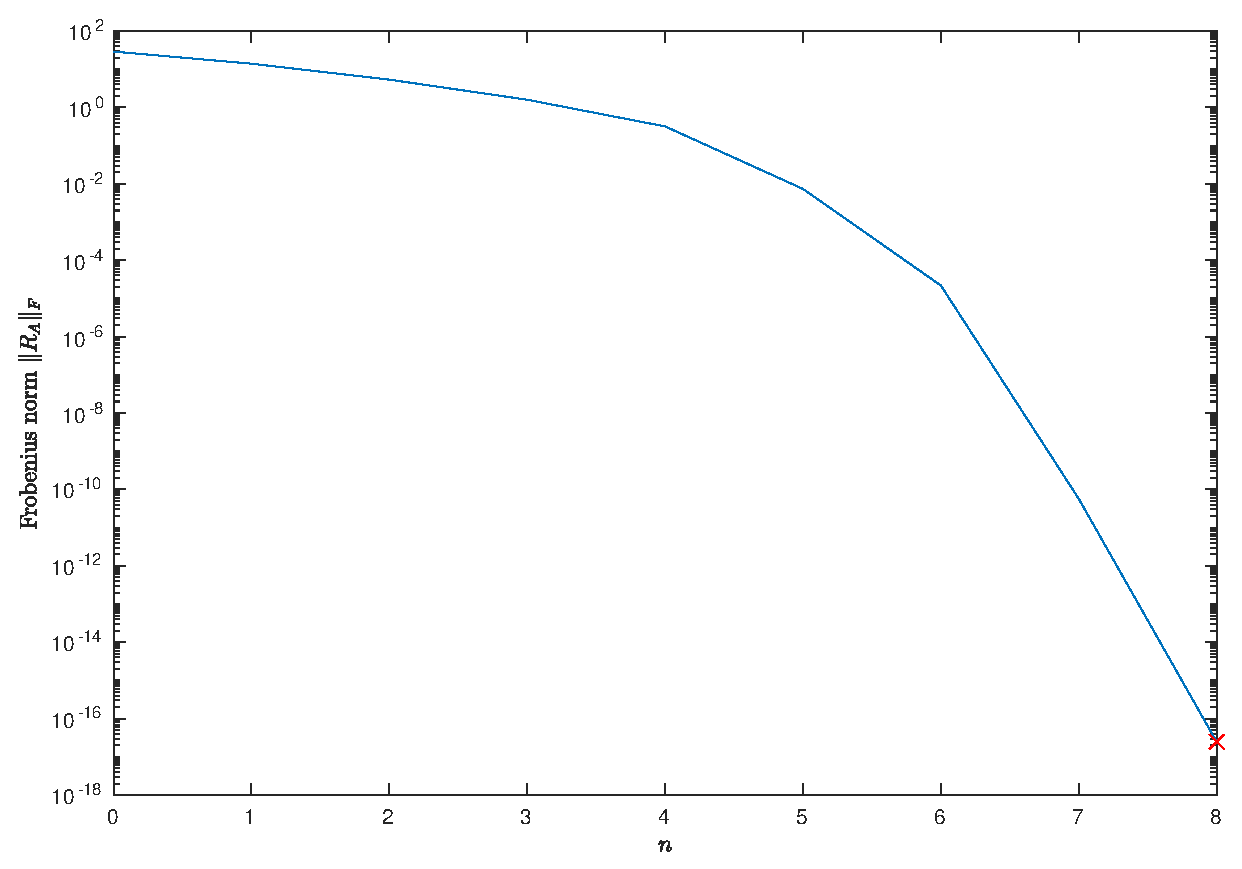
\includegraphics[scale=0.55]{../Afbeeldingen/fout-jacobiSweep.eps}
 \caption{Frobeniusnorm $\|R_A\|_F$ in functie van het aantal volledige $sweeps$ $n$}
 \label{fig:sweeps}
 \end{figure}
\newpage


\lstinputlisting[caption={jacobi.m}, label = {lst:jacobi}]{../Code/jacobi.m}

\section{Geconjugeerde gradi\"enten} \label{sec: geconjugeerde gradienten}
\underline{\textbf{Opgave 7a}}\\

Bij de methode van de conjugeerde gradi\"enten  toegepast op een positief definiete symmetrische matrix probleem $Ax = b$, met $\kappa(A)$ het conditiegetal van de matrix $A$, geldt de volgende ongelijkheid:
\begin{align}\label{eq:ongelijkheidCG}
\left.\frac{\|e_n\|_A}{\|e_0\|_A} \leq 2 \middle/ \left[ \left( \frac{\sqrt{\kappa(A)} + 1}{\sqrt{\kappa(A)} - 1}\right)^n + \left(\frac{\sqrt{\kappa(A)} + 1}{\sqrt{\kappa(A)} - 1}\right)^{-n}\right]\right. \leq 2\left(\frac{\sqrt{\kappa(A)} - 1}{\sqrt{\kappa(A)} + 1}\right)^n
\end{align}
Indien de waarden voor $\|e_0\|_A = 1$ en $\|e_{10}\|_A = 2^{-9}$ bekend zijn, kan er een ondergrens voor $\kappa(A)$ bepaald worden door vergelijking (\ref{eq:ongelijkheidCG}) in te vullen. Dit geeft volgende oplossing:
\begin{align*}
2\left(\frac{\sqrt{\kappa(A)} - 1}{\sqrt{\kappa(A)} + 1}\right)^{10} &\geq \frac{\|e_{10}\|_A}{\|e_0\|_A} = 2^{-9}\\
  \left(\frac{\sqrt{\kappa(A)} - 1}{\sqrt{\kappa(A)} + 1}\right)^{10} &\geq 2^{-10}\\
 \frac{\sqrt{\kappa(A)} - 1}{\sqrt{\kappa(A)} + 1} &\geq \frac{1}{2}\\
 2\sqrt{\kappa(A)} - 2 &\geq \sqrt{\kappa(A)} + 1\\
 \sqrt{\kappa(A)} &\geq 3\\
 \kappa(A) &\geq 9
 \end{align*}
 \underline{\textbf{Opgave 7b}}\\

 
Het conditiegetal $\kappa(A)$ heeft dus een ondergrens van 9. Deze ondergrens geeft geen extra informatie over $\|e_n\|_A$ voor $n$ groter dan 10. Wel kan uit volgende eigenschap:
\begin{align*}
\|e_n\|_A \leq \|e_{n-1}\|_A
\end{align*}
een bovengrens voor $\|e_{20}\|_A$ bepaald worden. 
\begin{align*}
\|e_{20}\|_A \leq \|e_{10}\|_A = 2^{-9}
\end{align*}
Een striktere bovengrens is niet mogelijk met de gegevens die ter beschikking zijn.
\end{document}